\chapter{El Problema: Juego de Distribuci\'on de la Cerveza}

%The purpose of the game is to understand the distribution side dynamics of a multi-echelon supply chain used to distribute a single item, in this case, cases of beer.


%There is a one-point cost for holding excess inventory and a one-point cost for any backlog (old backlog + orders - current inventory).

%The game is used to illustrate one of the links between System Dynamics theory and the Feedback Control Theory which inspired it - that systems with positive feedback loops and high gain can lead to oscillation and overload,

\section{Origen y Descripci\'on}

\textit{The Beer Distribution Game}, planteado por primera vez en la Escuela de Administraci\'on y Direcci\'on de Empresas Sloan del MIT en los años 60

\subsection{Principales caracter\'isticas}

La estructura se puede observar en la figura \ref{diagram_wikipedia}.\footnote{Imagen tomada de la página de Wikipedia \textit{The Beer Distribution Game}, bajo la licencia Creative Commons Attribution-Share Alike 3.0 Unported}\\


\begin{figure}[h]
\caption{Distribución de Cerveza}
\label{diagram_wikipedia}
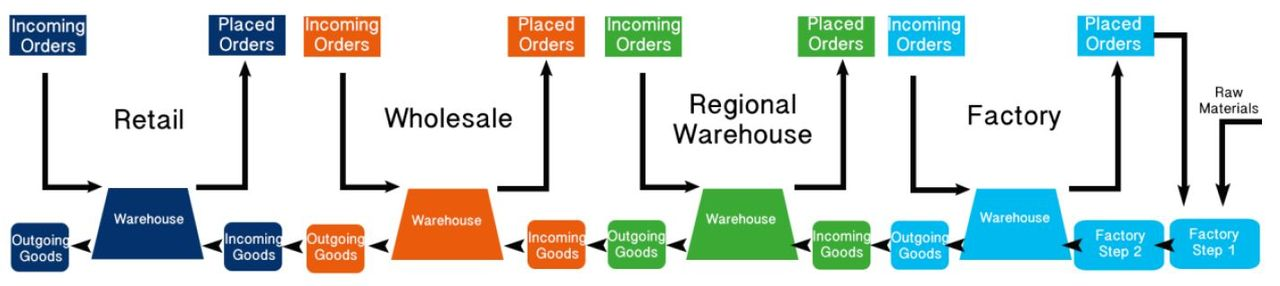
\includegraphics[width=8cm]{Diagrama_Wikipedia.JPG}
\centering
\end{figure}

Las variables globales que tienen efecto en este problema son:
\begin{itemize}
    \item Demanda del Consumidor
\end{itemize}


# Global variables

beer price          #cost per product unit
warehouse cost      #holding in warehouse per time unit per product unit
penalty fee         #backlog orders cost. 
                    #not fulfilling orders leave clients unhappy


# Agent variables

agent.inventory[t]  #what the agent has on the warehouse
agent.upstream[t]   #upstream orders.
                    #fulfilled immediately but constrained to have enough
agent.downstream[t] #downstream orders
agent.backlog[t]    #backlogged orders


Para cada uno de los agentes: tiendas minorista, mayorista y de distribución, y fábrica.\\


\subsection{Efecto Látigo}

El \textit{Efecto Látigo} se ejemplifica con el siguiente escenario:


\begin{enumerate}
    \item El comprador, que generalmente compra $6$ cervezas, ahora quiere $10$, pero la tienda minorista solamente cuenta con $7$. El minorista le venderá todo su inventario, pues es la acci\'on que maximiza su ganancia. Debe decidir si volverá a tener un inventario de $6$ o si debe pedir un número mayor de cervezas, atendiendo la aparentemente creciente demanda. Decide pedir $9$ cervezas al siguiente nivel, la tienda de mayoreo.
    \item El mayorista cuenta con $17$ cervezas. Llena el pedido del minorista, pero decide que ten\'ia guardado demasiado inventario, as\'i que se queda con $8$ cervezas en su almac\'en, sin hacer una orden al siguiente nivel, la tienda de distribución.
    \item La tienda de distribuci\'on decide no comprar unidades a la f\'abrica, dado que no disminuy\'o su inventario.
    \item La f\'abrica conoce la restricci\'on de estacionalidad de la cebada, as\'i que compra una m\'inima cantidad a los campos.
\end{enumerate}

En este escenario, el mayorista obtuvo informaci\'on distorsionada acerca del repentino crecimiento en la demanda del comprador, mientras que la tienda de distribución podr\'ia incluso interpretar que el comprador disminuy\'o su consumo. Si este comportamiento se mantiene durante algunos periodos más, recibiría la noticia (por medio de un incremento en las órdenes regulares) con un retraso considerable.\\

El \textit{Efecto L\'atigo} se refiere precisamente a este fenómeno: mientras m\'as ``arriba'' en la cadena de suministro se encuentre un agente (es decir, m\'as lejos del contacto directo con el comprador), m\'as distorsionada es la informaci\'on que tiene acerca de la verdadera demanda del comprador.

\section{Acercamiento en el Presente Trabajo}

Este problema se ha estudiado antes por \citet{Strozzi}, por medio de Algoritmos Genéticos y por \citet{Chaharsooghi} por medio de $Q-learning$. Ambas metodolog\'ias ser\'an abordadas en el siguiente cap\'itulo.\\

El aporte de este trabajo será agregar un componente de estacionalidad en el proveedor de la f\'abrica: el campo.